\section{Unsupervised debiasing by subgroup discovery}
\label{sec:unsupervised-end}

\begin{figure*}
    \centering
    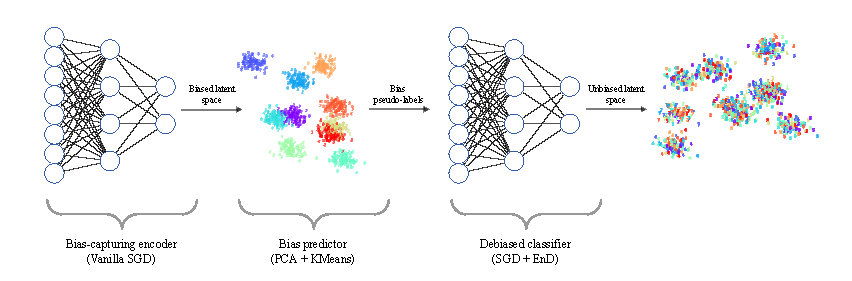
\includegraphics[width=\textwidth]{img/overview.pdf}
    \caption{Overview of our unsupervised debiasing approach: first we train a bias-capturing encoder, then we determine bias pseudo-labels with a bias predictor. Finally we employ the predicted labels for training a final debiased classifier. In this figure we use Biased MNIST~\cite{bahng2019rebias} as example, where the bias is given by a strong correlation between digit and color.}
    \label{fig:overview-unsupervised}
\end{figure*}

\begin{algorithm}
\DontPrintSemicolon
\SetKwBlock{stepA}{Train bias-capturing model}{end}
\SetKwBlock{stepB}{Train bias predictor}{end}
\SetKwBlock{stepC}{Train unbiased classifier}{end}
\KwIn{
    \begin{minipage}{.75\linewidth}
    Training and validation data $X^t = \{(x_i, y_i)\}$, $X^v = \{(\hat{x}_i, \hat{y}_i)\}$;
    Randomly initialized parameters $\theta_B = \{\theta_f, \theta_g\}$ and $\theta_D = \{\theta_f^D, \theta_g^D\}$ of the biased and unbiased classifiers.
    \end{minipage}
}
\BlankLine

\KwOut{Trained parameters $\theta_D$ of the unbiased classifier.}
\BlankLine

\stepA{
\par
Train the biased classifier using vanilla SGD: $\theta_B \leftarrow \text{SGD}(\theta_B, X^t)$\;
Compute the biased representations:
$Z^t = \{ f(x; \theta_f) \} \quad \forall x \in X^t$ and
$Z^v = \{ f(x; \theta_f) \}\quad\forall x \in X^v$\;
}

\stepB{
Compute the PCA projections $P^t, P^v$ of $Z^t,Z^v$\; 
Fit $k$ clusters on $P^v$ choosing the optimal $k$ based on silhoutte and compute the cluster centroids:
$\{\mu_1,...,\mu_k\} \leftarrow \text{KMeans}(P^v, k)$\;
Assign the pseudo-labels $\hat{b}_i \leftarrow \underset{b \leq k}{\arg\!\min}\,(P^t_i,\, \mu_b)$\; 
Update the training set $X^t \leftarrow \{(x_i, y_i, \hat{b}_i)\}$\;
}

\stepC{
Learn the parameters $\theta_D$ on $X^t$ searching the optimal $\alpha$ and $\beta$ on $X^v$:
$\theta_D \leftarrow \text{SGD}(\theta_D, X^t) + R(\theta^D_f, X^t, \alpha, \beta)$\;
}

\caption{General scheme of U-EnD}
\label{alg:overview}
\end{algorithm}

\noindent In this section we present our proposed unsupervised end-to-end debiasing approach, showing how an explicitly supervised technique such as EnD can be extended to the unsupervised case, where the bias labels are unavailable. 
We do this by showing how the bias information can be partially, and sometimes fully, recovered in a completely unsupervised manner. 
To achieve that, our proposed algorithm consists of three sequential steps, as illustrated in Fig.~\ref{fig:overview-unsupervised}. 
First, we train a bias-capturing classifier, employing standard optimization techniques (e.g. SGD or Adam);  
then, we recover bias-related information from the latent space of the biased classifier via clustering, in order to obtain a bias predictor, which we employ to categorize all of the training samples into different bias classes. Lastly, we apply the EnD debiasing technique using the predicted bias labels, in order to obtain a debiased classifier.
A general scheme of the entire pipeline can be found in Algorithm~\ref{alg:overview}. 
Throughout this work, we make the assumption that an \emph{unbiased} validation set is available: this is needed for searching the optimal EnD hyper-parameters.


\subsection{Training a bias-capturing model}
\label{sec:phase1}
The first step of our proposed algorithm is to train a bias-capturing model, which in our case is represented by a \emph{biased} encoder. To achieve this, we perform a vanilla training of a CNN classifier on the available training data. Here, we do not employ any technique aimed at dealing with the presence of biases in the data. The intuition of this approach is that 
if bias features are easier to learn than the desired target attributed, then the resulting model will also be biased. This has also been observed by other works. Following the definition proposed by Nam~\emph{et al.}~\cite{nam2020learning} we can identify two cases:

\begin{itemize}
    \item \emph{benign biases:} even if biases are present in the data, the model does not rely on bias related features as the target task is easier to learn;
    \item \emph{malignant biases:} biases are present in the data, and they are easier for the model to learn instead of the target task.
\end{itemize}

\noindent The latter case is the most relevant for our work, as malignant biases are those which result in a loss of performance when evaluating the model on an unbiased set.
Fig.~\ref{fig:overview-unsupervised} shows a visualization of the embeddings obtained with a biased encoder on the BiasedMNIST~\cite{bahng2019rebias} dataset, where the background color correlates very well with the target digit class, as shown in Fig.~\ref{fig:biased-mnist}.
It is clear how the different clusters emerging in the latent space correspond to the different background color, rather than to the actual digit.
This first step is summarized in Algorithm~\ref{alg:overview}, and we now provide a more formal description.
Let $\theta_B = \{\theta_f, \theta_g\}$ be the set of parameters of the bias-capturing model $p(x; \theta) = g(f(x; \theta_f); \theta_g)$ where $f$ and $g$ are the encoder and the classifier, respectively. The objective function we aim to minimize is the cross-entropy loss (CE):
\begin{equation}
    \label{eq:objective-fun-biased}
    \mathcal{L}_\text{CE}(p(x; \theta_B), q(x)) = -\sum_{t \in T} q(t|x) \log p(t|x;\theta_B)
\end{equation}
where $q(x)$ represents the ground truth class distribution. We say that there is a benign bias in the dataset, if we can identify some distribution $r(x)$, related to some other confounding factor in the data, such that there exists a set of parameters $\theta'$ which is a local minimizer of~\eqref{eq:objective-fun-biased} and
$\theta' = \arg\!\min_{\theta_B} \mathcal{L}_\text{CE}(p(x; \theta_B), r(x))$. 
If, additionally, $r(x)$ is also easier to approximate than $q(x)$, then the bias is malignant and by applying the optimization process we obtain a bias-capturing model.
Once the biased model is trained, we only consider the encoder $f(x; \theta_f)$, as we are interested in analyzing its latent space in order to retrieve bias-related information. 

\subsection{Fitting a bias predictor}
\label{sec:phase2}

The second step consists in obtaining a predictor which can identify the bias in the data. 
Based on the observations made in Section~\ref{sec:phase1}, we employ a clustering algorithm to categorize the extracted representations into different classes. As shown in Fig.~\ref{fig:overview-unsupervised}, the identified clusters correspond to the biases in the dataset.
In this work, we choose KMeans~\cite{lloyd1982least} as it is one of the most well-known clustering algorithms.
Given a set of representation $z = \{z_1, z_2,\dots, z_n\}$ extracted by $f(x; \theta_B)$ we aim to partition $z$ into $k$ sets $C = \{C_1, C_2, \dots, C_k\}$ in order to minimize the within-clusters sum of squares (WCSS), which can be interpreted as the distance of each sample from its corresponding cluster centroid, by finding: 
\begin{equation}
    \label{eq:kmeans-objective}
    \arg\!\min_C \sum_{i=1}^k \sum_{z \in C_i}|| z - \mu_i ||^2
\end{equation}
where $\mu_i$ is the centroid (average) of $C_i$.
Furthermore, once the clusters have been determined, 
it is very easy to use the determined centroids for classifying a new sample $\hat{z}$ based on its distance, simply by finding 
\begin{equation}
    \label{eq:kmeans-predict}
    \hat{b} = \arg\!\min_{i \leq k} ||\hat{z} - \mu_i||^2
\end{equation}
where $\hat{b}$ denotes the resulting pseudo-label. 
The KMeans algorithm requires a pre-specified number of clusters $k$: in this work, we automatically tune this parameter based on the
best silhouette score~\cite{rousseeuw87silhouetteCluster}, obtained by performing a grid search in the range $[2, 15]$. 
Considering that the representations obtained on the training set might be over-fitted, we choose to minimize \eqref{eq:kmeans-predict} on the validation set. Then, once the centroids of the clusters have been found, we use them for pseudo-labelling the training set.
Additionally, as KMeans is based on euclidean distance, which can yield poor results in highly dimensional spaces, we perform a PCA projection of the latent space before solving~\eqref{eq:kmeans-objective}~and~\eqref{eq:kmeans-predict}. For the same reasons as above, the PCA transformation matrix is also computed on the validation set.
We refer to the ensemble of the PCA+KMeans as \emph{bias predictor} model.
The cluster information is then used as bias pseudo-label, as explained in Section~\ref{sec:phase3}. 

\subsection{Training an unbiased classifier}
\label{sec:phase3}
The third and final step of our proposed framework consists in training an unbiased classifier using. For this purpose, we use the clusters discovered in the previous phase as pseudo-labels for the bias classes, as shown in Figure~\ref{fig:overview-unsupervised}. This allows us to employ the fully supervised EnD regularization term for debiasing. Here we follow the approach described in Section~\ref{sec:supervised-end}.
Denoting with $\theta_D = \{\theta_f^D, \theta_g^D\}$ the parameters of the encoder and the classifier of the debiased model $p'(x; \theta_D) = g(\gamma(f(x; \theta_f^D)); \theta_g^D)$.
The objective function that we aim to minimize in this phase is:
\begin{equation}
    \label{eq:objective-fun-unbiased}
    \mathcal{L}_\text{CE}(p'(x; \theta_D), q(x)) + R(\gamma(f(x; \theta_f^D)), q(x), b(x))
\end{equation}
where $b(x)$ is the distribution corresponding to the pseudo-labels computed in the clustering step of Section~\ref{sec:phase2}. The closer $b(x)$ is to the real distribution $r(x)$, the more minimizing~\eqref{eq:objective-fun-unbiased} will lead to minimizing $R$ with the respect to the unknown ground-truth bias labels.

\section{Analysis on controlled experiments}
\label{sec:analysis-mnist}

\begin{figure}
    \centering
    
\includegraphics[width=\columnwidth]{img/mnist.png}
    \caption{Biased MNIST by Bahng~\emph{et~al.} ~\cite{bahng2019rebias}. The bias is given by the correlation between digit and background color.}
    \label{fig:biased-mnist}
\end{figure}

In this section we provide more insights supporting the proposed solution. 
To aid in the explanation of the different steps of the algorithm, we employ the Biased-MNIST dataset~\cite{bahng2019rebias} as case study throughout this section. Biased-MNIST is built upon the original MNIST~\cite{lecun2010mnist} by injecting a color bias into the images background, as shown in Fig.~\ref{fig:biased-mnist}. 
A set of ten default colors associated with each image is determined beforehand. 
To assign a color to an image, the default color is chosen with a probability $\rho$, while any other color is chosen with a probability of $(1-\rho)$. 
More explicitly, given a label $i, 0 \leq i < N_T$ with $N_T=10$,
the probability distribution for each color is given by: 
\begin{equation}
    \begin{cases}
        P(B = i|T = i) = \rho \\
        P(B \neq i | T = i) = \frac{1}{N_T - 1} (1 - \rho)
    \end{cases}
    \label{eq:dist-b-given-t}
\end{equation}
where $B$ and $T$ are random variables associated to the bias and target class respectively.
The $\rho$ parameter allows us to determine the degree of correlation between background color (\emph{bias}) and digit class (\emph{target}). %
Hence, higher values of $\rho$ correspond to more difficult settings.
Following~\cite{bahng2019rebias}, we generate different biased training set, by selecting $\rho \in \{0.990, 0.995, 0.997, 0.999 \}$. In order to assess the generalization performance when training on a biased dataset, we construct an \emph{unbiased} test set generated with $\rho =\frac{1}{N_T} = 0.1$. Given the low correlation between color and digit class in the unbiased test set, models must learn to classify shapes instead of colors in order to reach a high accuracy. 

\begin{table}
    \centering
    \resizebox{\columnwidth}{!}{%
    \begin{tabular}{l c c c c}
        \toprule
        \multirow{2}{*}{Method} & \multicolumn{4}{c}{$\rho$ values}\\
                                & 0.999 & 0.997 & 0.995 & 0.990 \\ 
        \toprule
        Vanilla~\cite{bahng2019rebias} & 10.40\std{0.50} & 33.40\std{12.21} & 72.10\std{1.90} & \underline{89.10}\std{0.10} \\
        LearnedMixin~\cite{ClarkYZ19} & \underline{12.10}\std{0.80} & \underline{50.20}\std{4.50} & \underline{78.20}\std{0.70} & 88.30\std{0.70} \\
        EnD~\cite{tartaglione2021end} & \textbf{52.30}\std{2.39}    & \textbf{83.70}\std{1.03}  & \textbf{93.92}\std{0.35}  & \textbf{96.02}\std{0.08} \\
        \midrule
        HEX$^\dagger$~\cite{wang2018learning} & 10.80\std{0.40} & 16.60\std{0.80} & 19.70\std{1.90} & 24.70\std{1.60} \\
        RUBi$^\dagger$~\cite{cadene2019rubi} & 13.70\std{0.70} & 43.00\std{1.10} & \underline{90.40}\std{0.40} & \underline{93.60}\std{0.40}\\
        ReBias$^\dagger$~\cite{bahng2019rebias} & 22.70\std{0.40} & 64.20\std{0.80} & 76.00\std{0.60} & 88.10\std{0.60} \\
        U-EnD$^\dagger$ ($T$=80) & \underline{53.90}\std{4.03} & \underline{82.16}\std{0.63} & 74.39\std{0.43} & 88.05\std{0.16} \\
        U-EnD$^\dagger$ ($T$=10) & \textbf{55.29}\std{1.27} & \textbf{85.94}\std{0.33} & \textbf{92.92}\std{0.35} & \textbf{93.48}\std{0.06} \\
        \bottomrule
    \end{tabular}
    }
    \caption{Biased-MNIST accuracy on the unbiased test set. Techniques which can be used in an unsupervised way are denoted with $^\dagger$.}
    \label{table:mnist-results}
\end{table}

Experimental details are provided in the supplementary material. %
The results for Biased-MNIST are presented in Table~\ref{table:mnist-results}. We report the accuracy on the unbiased test set, obtained with the supervised EnD techique and the unsupervised extension. We also report reference results~\cite{bahng2019rebias} of other debiasing algorithms, both supervised and unsupervised. 
For U-EnD, we evaluate the results employing pseudo-labels computed at different training iterations ($T$) of the biased encoder: at an early stage after 10 epochs, and at a late stage at the end of training (80 epochs). In this section we focus on the late stage pseudo-labelling, while a detailed comparison between the two cases will be the subject of Section~\ref{sec:easy_first}.
Using the unsupervised method we are able to match the original performance of EnD with the ground-truth bias labels in most settings: this is true especially when the bias is stronger (higher $\rho$ values). This is because in these cases, the bias-capturing models will produce representations strongly biased towards the color, and the pseudo-labels obtained with the bias predictor model will be accurate. On the other hand, a slightly larger gap is observed when there is less correlation between target and bias features. 
This is the most difficult settings for the unsupervised clustering of the bias features: however, a significant improvement with respect to the baseline is always achieved. 
It may be argued that in such cases of weaker bias (or even absence of it), the representations extracted by the biased encoder will be more aligned with the target class rather the the bias features. In this case, the resulting pseudo-labels will be less representative of the actual bias, leading to the disentangling, instead, of the target labels. We identify two worst-case scenarios which might lead to inaccurate pseudo-labels: \emph{i.)} the training set is already unbiased, \emph{ii.)} the pseudo-labels we identify correspond to the target rather then to the bias labels. In this cases, applying a debiasing technique might lead to worse performance with respect to the baseline, however we are able to avoid this issue thanks to the hyper-parameters optimization policy that we employ. A more detailed analysis of the worst-case settings can be found in the supplementary material. %



\subsection{Easier patterns are preferred}
\label{sec:theoretical-model}

In this section we analyze how the bias affects the learning process, in order to provide a better understanding of the bias-capturing model.
By analyzing the training process at different values of $\rho$, we can identify when the color bias shifts from being benign to malignant. Fig.~\ref{fig:mnist-training} shows the training accuracy of vanilla models (the first step of our technique) trained with different values of $\rho$. Given that, in this case, the number of target classes and the number of different colors (bias classes) are the same, we are able to compute a bias \emph{pseudo-accuracy}
by finding the permutation of the predicted labels which maximizes the accuracy with respect to the ground truth bias labels: this gives value gives us an indication on how the final predictions of the model are aligned with the bias. 
From Fig.~\ref{fig:mnist-train} we observe that the target accuracy on the training set is, as expected, close to 100\%, while the bias accuracy is exactly the value of $\rho$, meaning that the models learned to recognize the digit.
This holds true also for the unbiased test set (Fig~\ref{fig:mnist-unbiased-test}), where the value $\rho=0.1$. However, if we focus on higher end of $\rho$ values (most difficult settings) as shown in Fig.~\ref{fig:mnist-unbiased-test-zoom}, we observe a rapid inversion in the trend: the target accuracy decreases, dropping to 10\% for $\rho=0.999$, while the bias accuracy becomes higher, close to 100\% towards the end of the $\rho$ range. In these settings, given the strong correlation between target and bias classes, it is clear that the bias has become easier for the model to learn, and thus malignant. These results can be viewed as further confirmation that neural networks tend to prefer and prioritize the learning of simpler patterns first, as noted by Nam~\emph{et~al.}~\cite{nam2020learning} and especially
Arpit~\emph{et~al.}~\cite{arpit2017memorization}: it is clear that, in order to be malignant, a bias must:

\begin{itemize}
    \item be an \emph{easier} pattern to learn that the target features;
    \item have a strong enough correlation with the target task.
\end{itemize}

\subsection{The effect of bias on learning}
\label{sec:bias-theoretical-model}
In order to provide a more in-depth understanding of the behaviour just described and to aid in the explanation of our debiasing technique, we propose a simple yet effective mathematical framework describing the impact of the bias on the learning process. 

Under the assumption that the target and biases classes are uniformly distributed across the dataset, we have:
\begin{align}
	H(T) &= -\sum_{i=1}^{N_T} P(t_i) \log_2 P(t_i) = \log N_T \nonumber \\
	H(B) &= -\sum_{j=1}^{N_T} P(b_j) \log_2 P(b_j) = \log N_T \label{eq:entropy_assumption}
\end{align}
where $T$ and $B$ are the random variables associated to the target and the bias class, respectively. Under the assumption of perfect learner, we must impose
   $H(Y|T) = 0$
(or in other words, the output $y_i$ of the model matches the ground truth value $t_i~\forall i$), and following the steps described in the supplementary material, %
we can write the \emph{normalized} mutual information
\begin{equation}
    \label{eq:MI_perfect}
	\widehat{I}_{perf}(B, Y) =  \log_{N_T}\left\{N_T\rho\left[\frac{1-\rho}{\rho(N_T-1)}\right]^{1-\rho}\right\}
\end{equation}
\begin{figure}
    \centering
    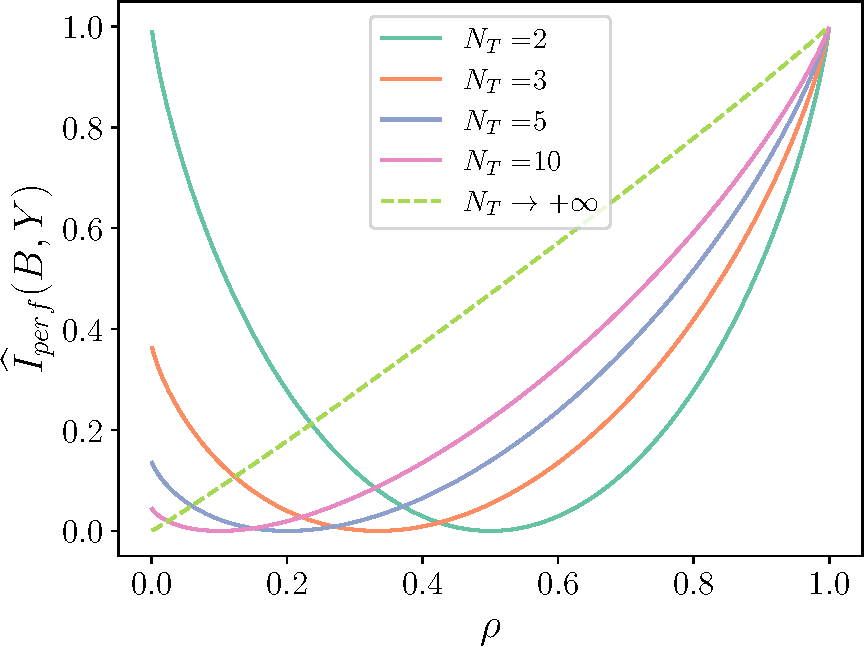
\includegraphics[width=\columnwidth]{img/MI_YZ.pdf}
    \caption{Normalized mutual information in case of perfect learner. As the number of classes $N_T$ increases, the curve smoothens. For low $N_T$ and low $\rho$ values, the anti-correlation phenomenon rises, and the mutual information increases.}
    \label{fig:MI_YZ}
\end{figure}
As it is possible to observe in Fig.~\ref{fig:MI_YZ}, a clear dependency between $\rho$ and \eqref{eq:MI_perfect} exists. In this case, the biased features and the target ones are in perfect overlap. Nonetheless, in the more general case the trained model is not a perfect learner, having $H(Y|T) \neq 0$.
The model, in this case, does not correctly classify the target for two reasons:
\begin{enumerate}
	\item It gets confused by the bias features, and it tends to learn to classify samples based on them. We model this tendency of learning biased features with $\phi$, which we call \emph{biasness}. The higher the biasness of is, the more the model relies on features which we desire to suppress, inducing bias in the model and for instance error in the model.
	\item Some extra error $\varepsilon$, non directly related to the bias features, which can be caused, for example, from stochastic unbiased effects, to underfit, or to other high-order dependencies between data. %
\end{enumerate}
We can write the discrete joint probability for $T, B, Y$, composed of the following terms.
\begin{itemize}
    \item When target, bias and prediction are aligned, the bias is aligned with the target class and correctly classified. Considering that we have not a prefect learner, we introduce the error term $\varepsilon$.
    \item When target and bias are align as well as bias and output, and the prediction is incorrect, it means that the model has not learned the correct feature and the bias is being contrasted.
    \item When target and bias are not aligned, but the prediction is correct and bias and output are aligned, it means that the model has learned the bias, introducing the error we target to minimize in this work.
    \item In all the other cases, the error of the model is due to higher-order dependencies, not directly related to the biasness $\phi$.
\end{itemize}
More formally, we can express the joint probability as:
\begin{align}
	P(T&,B,Y) = \frac{1}{N_T} \cdot \left[\delta_{tby} \rho (1 - \varepsilon) + \bar{\delta}_{ty}\delta_{tb}\delta_{by} \frac{(1-\phi)(1-\rho)}{N_T-1} \nonumber \right .\nonumber \\[1em]
	&+ \bar{\delta}_{tb}\delta_{ty}\delta_{by}\frac{\phi(1-\rho)}{N_T-1} + \delta_{tb}\bar{\delta}_{ty}\bar{\delta}_{by} \frac{\varepsilon \rho^2}{N_T-2+\rho} \nonumber \\[1em]
	&\left . + \bar{\delta}_{tb}\bar{\delta}_{ty}\bar{\delta}_{by} \frac{\varepsilon \rho (1-\rho)}{(N_T-1)(N_T-2+\rho)} \right]
    \label{eq:Pjointtotal}
\end{align}
where $\delta$ is the Kronecker delta function\footnote{for easiness of notation we suppress the index $i$: with $\delta_{tby}$ we implicitly intend that bias target and output are aligned to some $i$; hence $\delta_{ti}\delta_{bi}\delta_{yi}$}, $\bar{\delta}=1-\delta$ and $\phi,\varepsilon\in[0; 1]$.\footnote{not all the possible combinations are present in the joint probability \eqref{eq:Pjointtotal}: the missing combinations are  considered impossible, like having bias disaligned from the output but target aligned with the bias and with the output of the model (it would correspond to the case $\bar{\delta}_{by}\delta_{ty}\delta_{tb})$} We marginalize \eqref{eq:Pjointtotal} over $T$, obtaining
\begin{align}
	P(&B,Y) = \frac{1}{N_T} \cdot \left\{\delta_{by} [\rho (1 - \varepsilon) + \phi(1-\rho)] \right .\nonumber\\
	&\left .+ \bar{\delta}_{by}\left [\frac{(1-\phi)(1-\rho)}{N_T-1} + \frac{\rho\varepsilon}{N_T-2+\rho}\right ]\right\}
	\label{eq:joint_bz}
\end{align}
from which we compute the normalized mutual information
\begin{align}
    &\widehat{I}(B, Y) = \log_{N_T}\left[\rho (1 - \varepsilon) + \phi(1-\rho)\right]^{\rho (1 - \varepsilon)+ \phi(1-\rho)}\nonumber\\
    &+ \log_{N_T} \left [\frac{(1-\phi)(1-\rho)}{N_T-1} + \frac{\rho\varepsilon}{N_T-2+\rho}\right ]^{(1-\phi)(1-\rho) + \frac{(N_T-1)\rho\varepsilon}{N_T-2+\rho}}\nonumber\\
    &+ 1 + \rho\varepsilon \left(\frac{N_T-1}{N_T-2-\rho} -1 \right)\label{eq:MIcool}
\end{align}
\begin{figure}
    \centering
    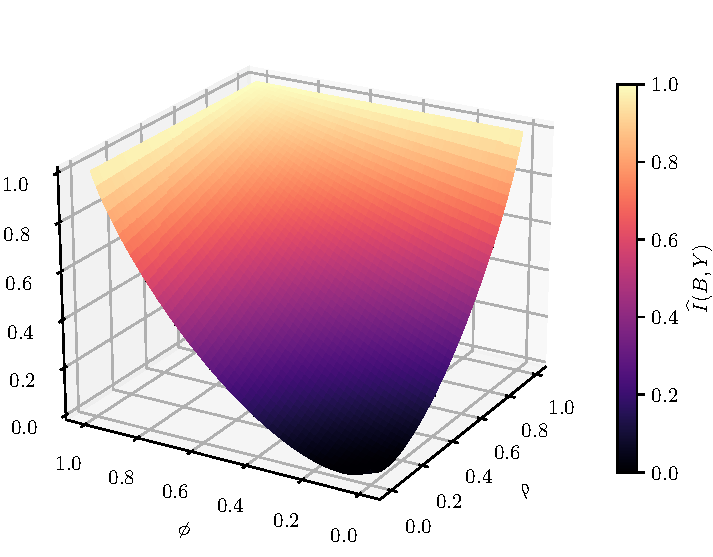
\includegraphics[width=1.0\columnwidth,trim={0 0 0 30},clip]{img/MI_YZ_full.pdf}
    \caption{Normalized mutual information between B and Y, in the case $\varepsilon=0$ and $N_T=10$. In light black, on top of the graph, level curves are drawn. In high $\rho$ regions, the mutual information is high regardless the bias tendency $\phi$ value, motivating the difficulty in learning the disentangling from biased features. A projection to a lower $\rho$ makes the problem of minimizing $\phi$ can drive the disentangling.}
    \label{fig:MI_YZ}
\end{figure}
The complete derivation can be found in the supplementary material %
and the plot for \eqref{eq:MIcool} in the case $\varepsilon=0$ is displayed in Figure~\ref{fig:MI_YZ}. 
Interestingly, we observe that for high values of $\rho$, the mutual information between the features
learned by the model and the bias is high, independently from the biasness $\phi$.
Typical learning scenarios, indeed, work in this region, where it is extremely challenging to optimize over $\phi$. On the contrary, with a lower $\rho$, the effect of $\phi$ appears evident. Towards this end, relying on a (relatively small) balanced validation set (hence, with low $\rho$) is extremely important in order to enhance the lowering of $\phi$. Directly optimizing over $\phi$ is in general not a duable strategy as the mutual information between B and Z in the typical training scenarios is very high; hence while bias removal can succeed, it will be extremely difficult to disentangle the biased features from the unbiased ones, without harming the performance.











\begin{figure*}
    \begin{subfigure}{0.33\textwidth}
        \centering
        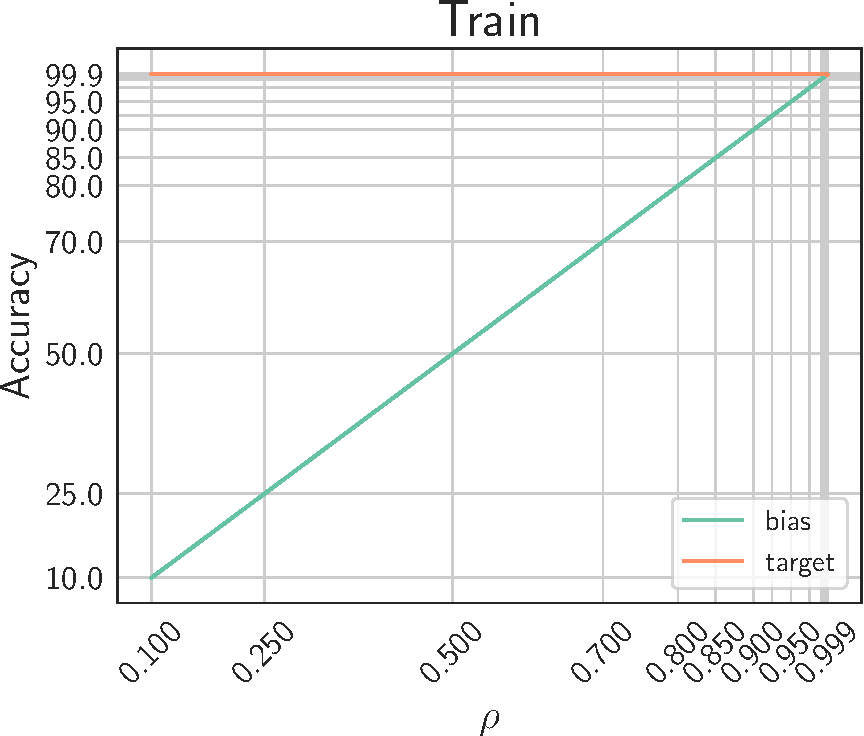
\includegraphics[width=\columnwidth]{img/mnist/train.pdf}
        \caption{~}
        \label{fig:mnist-train}
    \end{subfigure}
    \hfill
        \begin{subfigure}{0.33\textwidth}
        \centering
        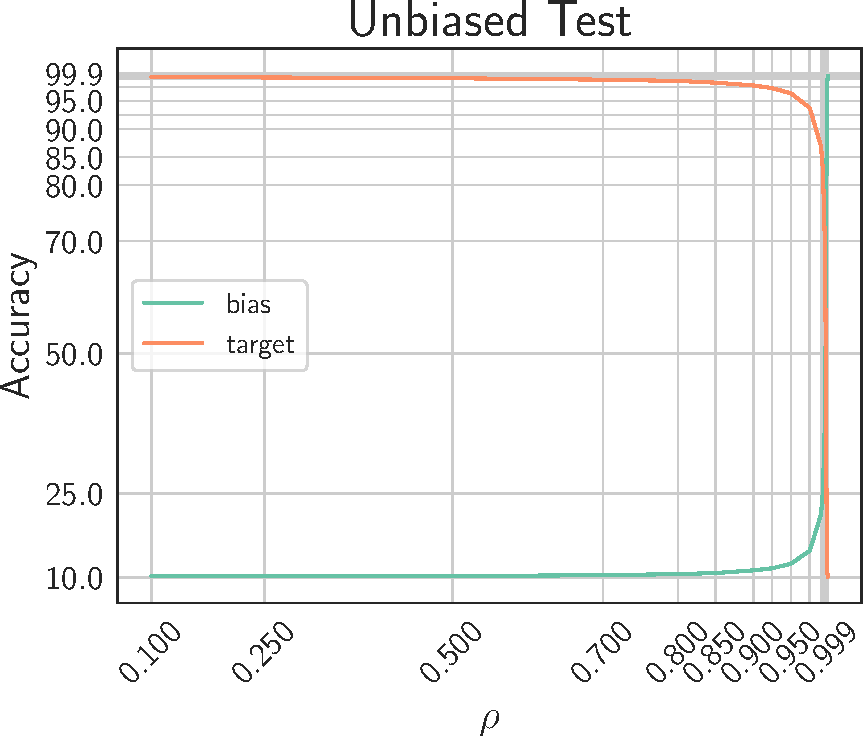
\includegraphics[width=\columnwidth]{img/mnist/unbiased_test.pdf}
        \caption{~}
        \label{fig:mnist-unbiased-test}
    \end{subfigure}
    \hfill
    \begin{subfigure}{0.33\textwidth}
        \centering
        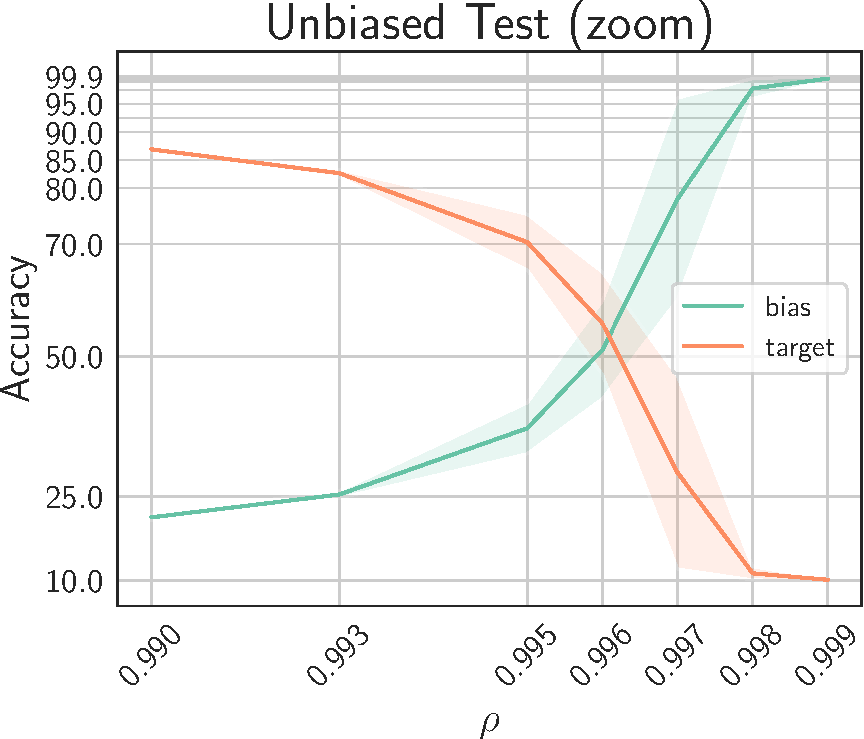
\includegraphics[width=\columnwidth]{img/mnist/unbiased_test_zoom.pdf}
        \caption{~}
        \label{fig:mnist-unbiased-test-zoom}
    \end{subfigure}
    
    \caption{Biased-MNIST accuracy on the training set (a), and on the unbiased test set (b) and (c). Results are reported in terms of mean and std across three different runs for every value of $\rho$. Given that the number of bias classes (colors) and target classes (digit) is the same, we can compute the bias accuracy by finding the permutation of predicted labels which maximizes the overlap with the ground truth bias labels.}
    \label{fig:mnist-training}
\end{figure*}

\subsection{Easier patterns are learned first}
\label{sec:easy_first}
Besides being easier to learn than the target task, we also find that biases tend to be learned in the first epochs. This is also evident when looking at the results in Table~\ref{table:mnist-results}, with $T=10$: using an early bias predictor results in more precise pseudo-labels, especially when $\rho$ is lower. In order to measure how biased the encoder is, we employ the theoretical model we presented in Eq.~\eqref{eq:joint_bz} to compute $\phi$ (the derivation can be found the supplementary material). %
In Fig.~\ref{fig:bias-tendency} we show the mean value of $\phi$ measured at different training iterations (we assume $\varepsilon=0$). As expected, the models tend to show stronger tendency towards bias when $\rho$ is higher. Interestingly, looking at the dynamics it is also clear that this behavior is exhibited predominantly in earlier epochs.
Under certain conditions, i.e. when the correlation between target and bias is not as strong, it is possible for the optimization process to escape the local minimum corresponding to a biased model. These findings are also confirmed by the related literature~\cite{nam2020learning, arpit2017memorization}. 

\begin{figure*}
    \centering
    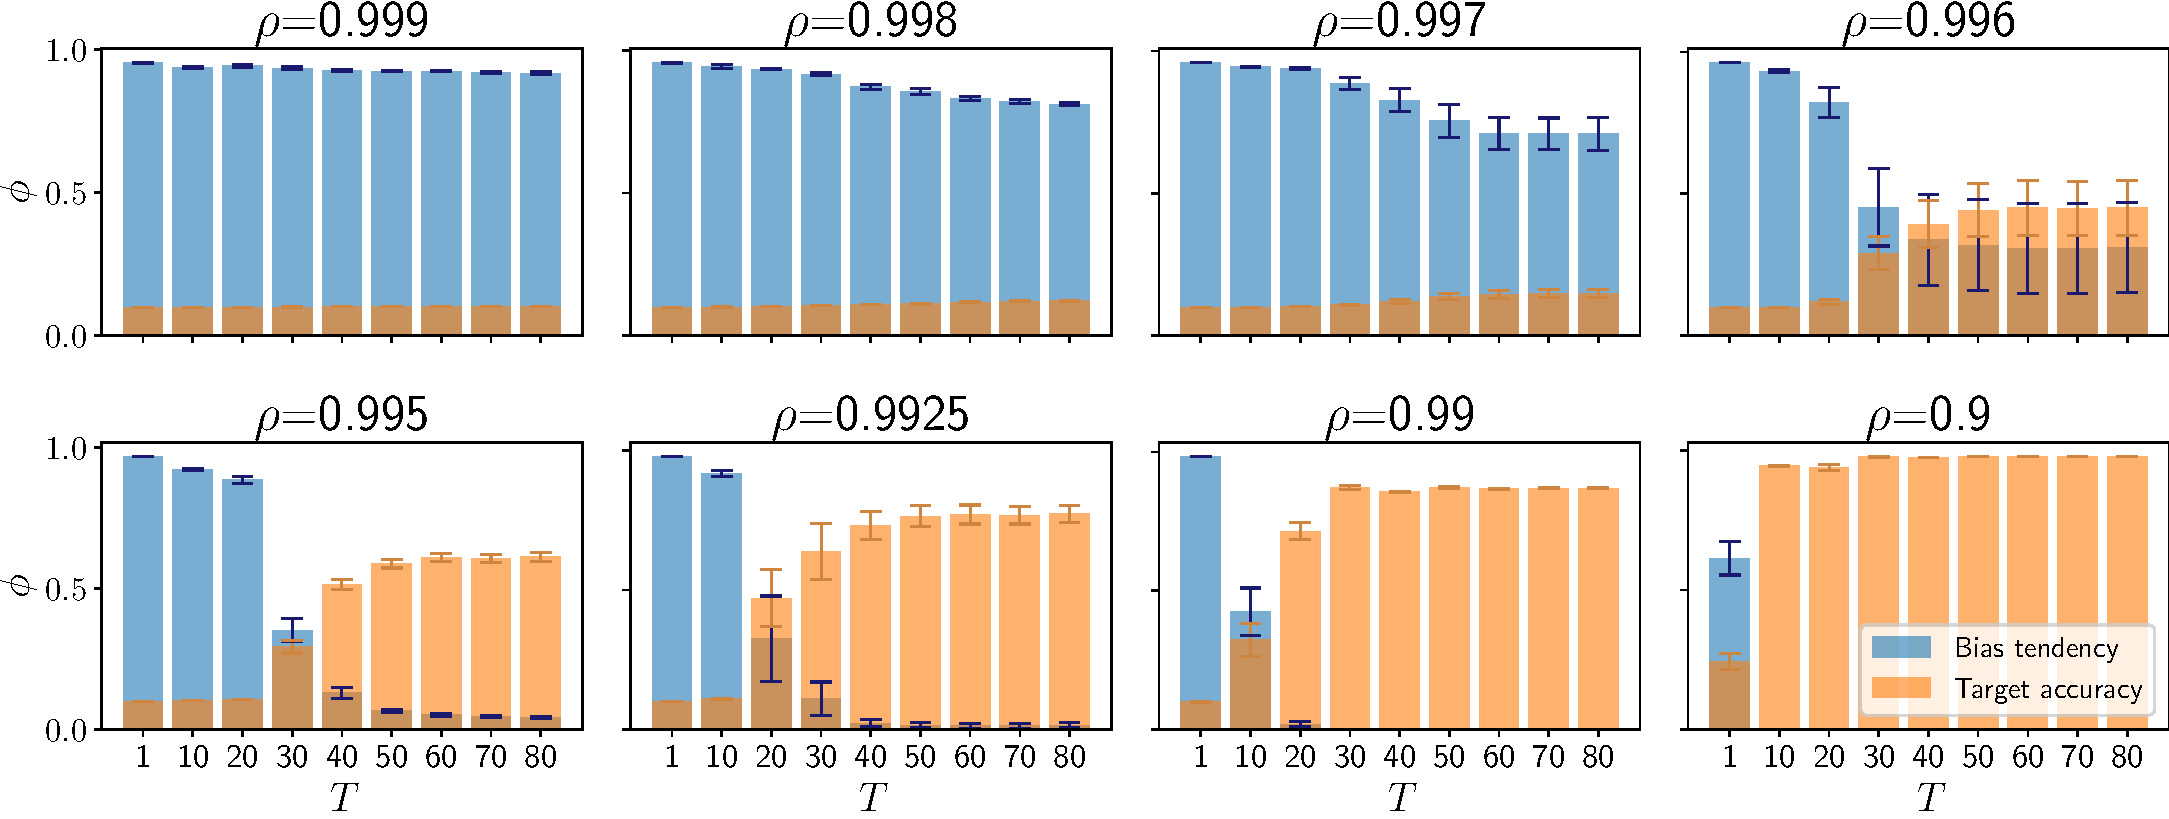
\includegraphics[width=\textwidth]{img/v.pdf}
    \caption{Biasness ($\phi$), or tendency towards learning bias features, in terms of mean and std computed across three independent runs for different values of $\rho$.}
    \label{fig:bias-tendency}
\end{figure*}


